\documentclass[a4paper,12pt]{scrartcl}
\usepackage{etex}
\usepackage{xltxtra}
\usepackage[babelshorthands]{polyglossia}
\usepackage{graphicx}
\usepackage{color}
\usepackage{hyperref}
\usepackage{amsmath}
\usepackage{unicode-math}
\setmathfont{XITS Math}

\usepackage{moreenum}

\typearea{18}
 
\pagestyle{empty}
\definecolor{linkcol}{rgb}{0.00,0.00,0.50}
\definecolor{urlcol}{rgb}{0.50,0.00,0.00}
\hypersetup{%
  pdftitle={Bildgenerierung, WS 2015/2016},
  pdfauthor={Holger Arndt},
  pdfpagemode=UseThumbs,
  colorlinks=true,
  linkcolor=linkcol,
  urlcolor=urlcol,
}

\setmainlanguage{german}
\defaultfontfeatures{Mapping=tex-text,Scale=MatchLowercase}
\setmainfont[Scale=1]{XITS}
\setsansfont[Scale=0.9]{FreeSans}
\setmonofont[Scale=0.82]{DejaVu Sans Mono}

\renewcommand{\theenumi}{\alph{enumi}}
\renewcommand{\labelenumi}{\theenumi)}

\newcommand{\pmat}[1]{\begin{pmatrix}#1\end{pmatrix}}

\begin{document}
 
\section*{Lösung zu Hermite-Kurven mit Schleife}

% GNUPLOT: LaTeX picture with Postscript
\begingroup
  \makeatletter
  \providecommand\color[2][]{%
    \GenericError{(gnuplot) \space\space\space\@spaces}{%
      Package color not loaded in conjunction with
      terminal option `colourtext'%
    }{See the gnuplot documentation for explanation.%
    }{Either use 'blacktext' in gnuplot or load the package
      color.sty in LaTeX.}%
    \renewcommand\color[2][]{}%
  }%
  \providecommand\includegraphics[2][]{%
    \GenericError{(gnuplot) \space\space\space\@spaces}{%
      Package graphicx or graphics not loaded%
    }{See the gnuplot documentation for explanation.%
    }{The gnuplot epslatex terminal needs graphicx.sty or graphics.sty.}%
    \renewcommand\includegraphics[2][]{}%
  }%
  \providecommand\rotatebox[2]{#2}%
  \@ifundefined{ifGPcolor}{%
    \newif\ifGPcolor
    \GPcolortrue
  }{}%
  \@ifundefined{ifGPblacktext}{%
    \newif\ifGPblacktext
    \GPblacktexttrue
  }{}%
  % define a \g@addto@macro without @ in the name:
  \let\gplgaddtomacro\g@addto@macro
  % define empty templates for all commands taking text:
  \gdef\gplbacktext{}%
  \gdef\gplfronttext{}%
  \makeatother
  \ifGPblacktext
    % no textcolor at all
    \def\colorrgb#1{}%
    \def\colorgray#1{}%
  \else
    % gray or color?
    \ifGPcolor
      \def\colorrgb#1{\color[rgb]{#1}}%
      \def\colorgray#1{\color[gray]{#1}}%
      \expandafter\def\csname LTw\endcsname{\color{white}}%
      \expandafter\def\csname LTb\endcsname{\color{black}}%
      \expandafter\def\csname LTa\endcsname{\color{black}}%
      \expandafter\def\csname LT0\endcsname{\color[rgb]{1,0,0}}%
      \expandafter\def\csname LT1\endcsname{\color[rgb]{0,1,0}}%
      \expandafter\def\csname LT2\endcsname{\color[rgb]{0,0,1}}%
      \expandafter\def\csname LT3\endcsname{\color[rgb]{1,0,1}}%
      \expandafter\def\csname LT4\endcsname{\color[rgb]{0,1,1}}%
      \expandafter\def\csname LT5\endcsname{\color[rgb]{1,1,0}}%
      \expandafter\def\csname LT6\endcsname{\color[rgb]{0,0,0}}%
      \expandafter\def\csname LT7\endcsname{\color[rgb]{1,0.3,0}}%
      \expandafter\def\csname LT8\endcsname{\color[rgb]{0.5,0.5,0.5}}%
    \else
      % gray
      \def\colorrgb#1{\color{black}}%
      \def\colorgray#1{\color[gray]{#1}}%
      \expandafter\def\csname LTw\endcsname{\color{white}}%
      \expandafter\def\csname LTb\endcsname{\color{black}}%
      \expandafter\def\csname LTa\endcsname{\color{black}}%
      \expandafter\def\csname LT0\endcsname{\color{black}}%
      \expandafter\def\csname LT1\endcsname{\color{black}}%
      \expandafter\def\csname LT2\endcsname{\color{black}}%
      \expandafter\def\csname LT3\endcsname{\color{black}}%
      \expandafter\def\csname LT4\endcsname{\color{black}}%
      \expandafter\def\csname LT5\endcsname{\color{black}}%
      \expandafter\def\csname LT6\endcsname{\color{black}}%
      \expandafter\def\csname LT7\endcsname{\color{black}}%
      \expandafter\def\csname LT8\endcsname{\color{black}}%
    \fi
  \fi
  \setlength{\unitlength}{0.0500bp}%
  \begin{picture}(4520.00,4520.00)%
    \gplgaddtomacro\gplbacktext{%
    }%
    \gplgaddtomacro\gplfronttext{%
    }%
    \gplbacktext
    \put(0,0){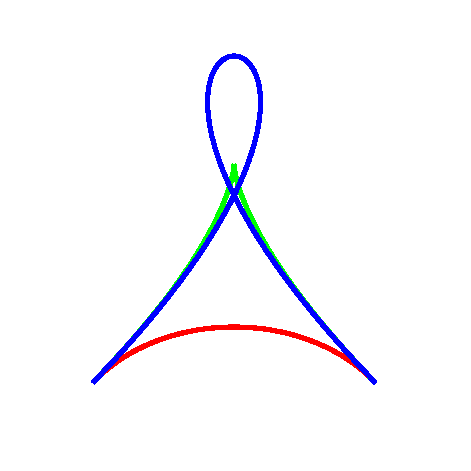
\includegraphics{hermiteTypen}}%
    \gplfronttext
  \end{picture}%
\endgroup


o.\,B.\,d.\,A.\ $a = 0$

\[ Q(t)_{x,y} = \pmat{ 0 & b & ρ & ρ \\ 0 & 0 & ρ & -ρ} ·
\pmat{2 & -3 & 0 & 1 \\ -2 & 3 & 0 & 0 \\ 1 & -2 & 1 & 0 \\ 1 & -1 & 0 & 0} ·
\pmat{t³ \\ t² \\ t \\ 1}
= \pmat{-2b + 2ρ & 3b - 3ρ & ρ & 0 \\ 0 & -ρ & ρ & 0} ·
\pmat{t³ \\ t² \\ t \\ 1} \]

Spitze (beim Übergang zur Schleife) für $Q'\left(\frac12\right) = 0$:

\begin{align*}
  x'(t) &= -6bt² + 6ρt² + 6bt - 6ρt + ρ \\
  y'(t) &= -2ρt + ρ
\end{align*}

\begin{align*}
  x'\left(\frac12\right) &= -\frac32 b + \frac32 ρ + 3b - 3ρ + ρ =
  \frac32 b -\frac12 ρ \\
  y'\left(\frac12\right) &= 0
\end{align*}

\[ x'\left(\frac12\right) = 0 ⇔ ρ = 3b \]

\end{document}
